%%%%%%%%%%%%%%%%%%%%%%%%%%%%%%%%%%%%% BEGIN HEADERS %%%%%%%%%%%%%%%%%%%%%%%%%%%%%%%%%%%%%%%%%%%%%%%%%%%%%
\documentclass[11pt,conference]{IEEEtran}

\usepackage{longtable}
\usepackage{graphicx}
\usepackage[utf8]{inputenc}
\usepackage{fancyhdr}
\usepackage{float}
\usepackage[hidelinks]{hyperref}
\usepackage{listings}
\usepackage{color}
\usepackage{natbib}
\usepackage{amsmath}

% Your names in the header
\pagestyle{fancy}
\rhead{Enrico Tedeschi}
\lhead{INF-3201 Parallel Programming - Assignment 3}
\cfoot{\thepage}

% Used for including code in a stylized manner
\definecolor{codegreen}{rgb}{0,0.6,0}
\definecolor{codegray}{rgb}{0.5,0.5,0.5}
\definecolor{codepurple}{rgb}{0.58,0,0.82}
\definecolor{backcolour}{rgb}{0.95,0.95,0.92}
 

\lstdefinestyle{mystyle}{
    backgroundcolor=\color{backcolour},   
    commentstyle=\color{codegreen},
    keywordstyle=\color{magenta},
    numberstyle=\tiny\color{codegray},
    stringstyle=\color{codepurple},
    basicstyle=\footnotesize,
    breakatwhitespace=false,         
    breaklines=true,                 
    captionpos=b,                    
    keepspaces=true,                 
    numbers=left,                    
    numbersep=5pt,                  
    showspaces=false,                
    showstringspaces=false,
    showtabs=false,                  
    tabsize=2
}

\lstset{style=mystyle}

% The Title
\title{INF-3201 Parallel Programming -- GPGPU}

% Your name and email
\author{\textbf{Enrico Tedeschi}\\ ete011@post.uit.no }


%%%%%%%%%%%%%%%%%%%%%%%%%%%%%%%%%%%%% END HEADERS %%%%%%%%%%%%%%%%%%%%%%%%%%%%%%%%%%%%%%%%%%%%%%%%%%%%%

\begin{document}

% Create the title and everything
\maketitle

\section{Introduction}
The goal of this assignment is to parallelize the given piece of code with \textbf{CUDA/OpenCL} and multiprocessing (combined).

\subsection{Requirements}
\begin{itemize} 
\item Parallelize an encrypt/decrypt code given
\item Use multiple cores on the CPU, and GPU, at the same time
\item The CPU parallel implementation can use shared memory or message passing models
\item Parallelize it with CUDA/OpenCL
\item Analyse the solution using the Nvidia Visual Profiler (if using CUDA)
\end{itemize}


\section{Technical Background}

\begin{itemize} 
\item[--] Concurrency and parallelism concepts
\item[--] Parallel programming concepts
\item[--] Basic programming approach
\item[--] Notion of GPU programming approach 
\item[--] Knowledge of C language
\item[--] Knowledge of Python language
\item[--] Notion of design pattern principles
\item[--] Theory about software engineering
\item[--] Knowledge of git to manage the software versions
\end{itemize}

\section{Analysis}
\subsection{Precode}
To solve the problem a deep analysis of the precode is required.
The given sequential code is written in \textit{Python} and it consists of three classes: \textit{precode.py}, \textit{decrypt.py} and \textit{encrypt.py}. The precode class is the one which does all the encryption and decryption work while the other two manage the input file to encrypt/decrypt and which kind of password to give. Since the decryption consists in a brute-force guessing password method, it has a terrible computational time and with a password of three characters it already runs out of memory.
\newline
\begin{figure}[h!]
  \centering
    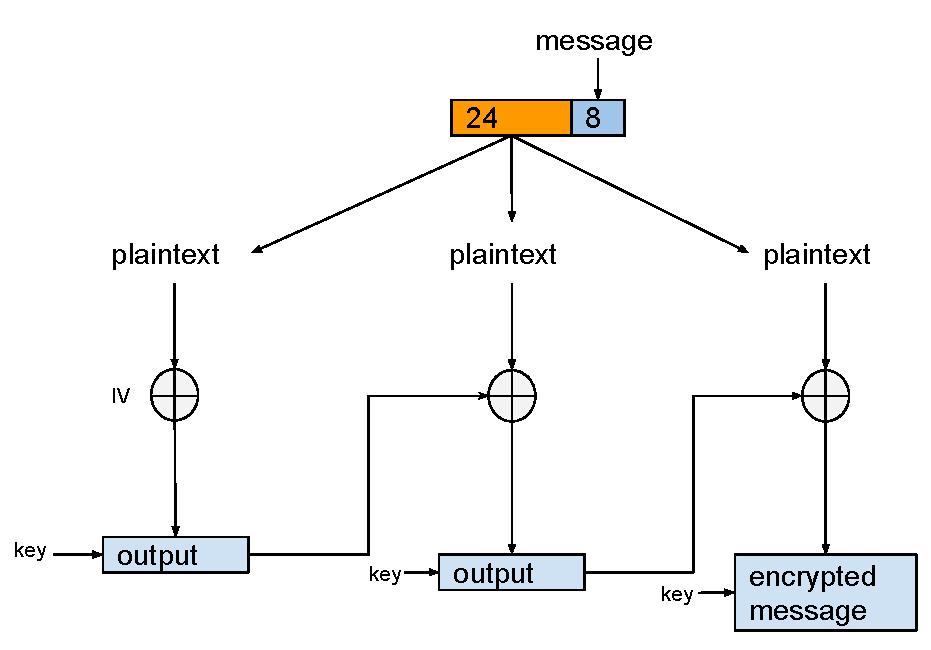
\includegraphics[width=0.5\textwidth]{encryption}
    \caption{XTEA and CBC encryption scheme}
    \label{fig:encryption}
\end{figure}

The Fig \ref{fig:encryption} shows how the encryption works. It takes the message as input and it generates from it a \textit{numpy array}. The array is made of 32 bits, 8 to contain the shuffled message and the other 24 tell about the right location of the shuffled message. To generate the first encrypted output the plaintext is enciphered using the key(which is an md5 of the current password) and the initial Instance Vector. The generated output becomes the new IV in the next iteration.
\[
C_i = E_k(P_i \oplus C_{i-1}), C_0 = IV
\]
In the formula $P$ is the plaintext and $E_k$ is the encryption method using the key \cite{CBC}.
\newline
The decryption works in the same way. The program tries to decrypt the message every time with a different key, and if in the text obtained it occurs the \textit{known\_text}, then the current key is the right password.
\subsection{Profiling}
The profiling of the precode was done on the \textit{ifilab110} machine and it shows that the most expensive function in matter of time computation is \textit{decipher()}, since the total execution time with a one character password is 15 seconds.
\begin{lstlisting}
ncalls  tottime filename:lineno(function)
55000   13.794  precode.py:215(decipher)
\end{lstlisting}

\subsection{Programming in C CUDA}
A good analysis of the C CUDA language is needed before starting the implementation, especially if you're new in GPU's programming. An important thing to consider is how the cuda kernel works with the variables. Every variable created in the CPU which is supposed to be used on the GPU must be allocated first in the GPU's memory, then initialized with a copy \textit{from host to device}; once the GPU is done the variable space must be deallocated and it returns free and the output variables have to be copied \textit{from device to host}. To simplify this process and to get an easy access to the CUDA API, \textbf{PyCuda} has been used. With it is possible to avoid the memory allocation part and manage directly the input and output variables. The function in the cuda kernel shouldn't have any return value since each variable is passed using the \textbf{HtoD} or \textbf{DtoH} copy.
\newline
To rewrite the code from \textit{Python} to \textit{C cuda} a deep analysis on the variable type has been done. These are the main types used in Python with the respective value in C cuda:

\begin{center}
    \begin{tabular}{ | l | l |}
    \hline
    \textbf{Python} & \textbf{C cuda} \\ \hline
    long & unsigned long \\ \hline
    int & unsigned int \\ \hline
    numpy.ndarray & unsigned int * \\ \hline
    numpy.uint32 & unsigned int \\ \hline
    \end{tabular}
\end{center}

With GPUs a relevant number of threads could be used in parallel. The structure of an nVidia GPU includes a grid where an uni-dimensional, bi-dimensional or three-dimensional block list could be declared. Each block could contain as well a 1D, 2D or 3D thread list, with a maximum number of 1024 threads per block.
%TODO: Talk about how gpu works with blocks and threads

\subsection{Possible Optimizations}
For every key guess the message is split in 1000 parts. The decipher function is executed for every piece of the message; consider that, the first implementation of the parallel version could be done parallelizing, for each key, the decipher for each part of the message (Fig \ref{fig:parallel_sol_1}).
\begin{figure}[h!]
  \centering
    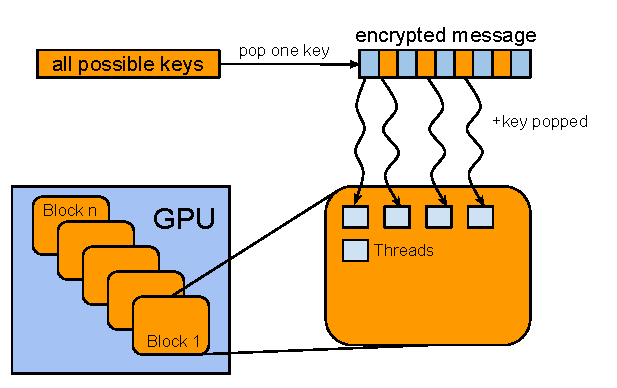
\includegraphics[width=0.5\textwidth]{parallel_sol_1}
    \caption{Possible 'easy' parallel solution}
    \label{fig:parallel_sol_1}
\end{figure}

The speedup wouldn't probably be that much by parallelizing only on the message length, since the most expensive part in matter of computation time to deal with is the huge amount of possible key combination. Good could be hence, to get the threads work at the same time on different keys (Fig \ref{fig:parallel_sol_2}).
\begin{figure}[h!]
  \centering
    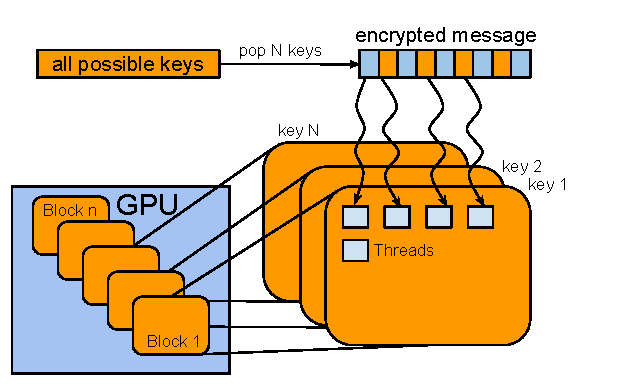
\includegraphics[width=0.5\textwidth]{parallel_sol_2}
    \caption{An harder way of getting a parallel solution}
    \label{fig:parallel_sol_2}
\end{figure}


%TODO: Talk about the variable malloc and PyCuda and show a table of the variable type traslation
\section{Implementation}

%TODO: Describe your algorithms

%TODO: Talk about CPU and GPU part

%TODO: Reasons for choosing this approach
\subsection{Environment}
The code has been developed using JetBrains CLion 1.1 on Windows 10 and the git control of version has been done on an Ubuntu Virtual Machine. The compilation and the execution of the code has been made on a dedicated machine in \textit{ifilab}. That due to a lack of NVidia graphic unit in my local computer.
\newline
To synchronize the ifilab machine and the local computer and to keep trace of all the changes in the code, a git repository was created and the git command on linux were used to commit and to push/pull data from repositories.
\newline
The benchmarking and the test were made on the \textit{ifilab110} machine. The connection with the remote machine was established by using PuTTY on Windows.


\subsection{Parallelization}

\section{Result and Benchmarking}


\subsection{Speedup}
\[ S(p) = \dfrac{t_s}{t_p}  \]
where $t_s$ is the sequential time and $t_p$ is the parallel time using p processors. 

 
\subsection{Efficiency}
\[ S(p) = \dfrac{t_s}{t_p * p}  \]
where p is the number of processes used. So the question which efficiency answers is: \textit{"How good is the parallelization using p number of cores?"}. 

\subsection{Scaling}

\section{Discussion}
%TODO: Critical rewiew of achieved performance

\section{Conclusion}

\bibliographystyle{plain}
\bibliography{report}


\end{document}

